\documentclass[12pt]{report}

\usepackage{amsfonts}
\usepackage{enumitem}
\usepackage{float}
\restylefloat{table}
\restylefloat{figure}

\usepackage[margin=1.5in]{geometry}
\usepackage{graphicx}

\usepackage{setspace}
\doublespacing

\usepackage{titlesec}
\titleformat{\chapter}[display]
    {\normalfont\huge\bfseries}{\chaptertitlename\ \thechapter}{0pt}{\Huge}
\titlespacing*{\chapter}{0pt}{0pt}{10pt}

\bibliographystyle{apalike}

\makeatletter
\renewcommand*\l@chapter[2]{
    \ifnum \c@tocdepth >\m@ne
    \addpenalty{-\@highpenalty}
    \addvspace{1.0em \@plus\p@}
    \setlength\@tempdima{1.5em}
    \begingroup
    \parindent \z@ \rightskip \@pnumwidth
    \parfillskip -\@pnumwidth
    \leavevmode
    \advance\leftskip\@tempdima
    \hskip -\leftskip
    #1\nobreak
    \xleaders\hbox{$\m@th
    \mkern \@dotsep mu\hbox{.}\mkern \@dotsep mu$}
    \hfil\nobreak\hb@xt@\@pnumwidth{\hss #2}\par
    \penalty\@highpenalty
    \endgroup
    \fi
}
\makeatother

\begin{document}

\pagenumbering{roman}

\tableofcontents

%% keep lof and lot on same page
\begingroup
\addcontentsline{toc}{chapter}{List of Figures}
\listoffigures

\let\clearpage\relax
\addcontentsline{toc}{chapter}{List of Tables}
\listoftables
\endgroup

\newpage

\addcontentsline{toc}{chapter}{Summary} %% 1 page

\paragraph This report, titled Learning Styles of a Computer Science Student, provides a short overview of some popular learning styles models and theories in the world, analyzes suitability of Kolb's Model to a computer science student, as well as Honey and Mumford's variation on the Kolb system.
    
\paragraph Three conclusions are reached in this report. First, a typical learning process of a computer science student could be described by Kolb's four stages learning theories. This is concluded from three common scenes of a computer science student. Second, any stage in a learning model might be entered firstly to achieve productive learning, as long as all four stages are covered. This is gained by extracting the steps of learning process. The author also concluded learning styles will change over time based on the statement from Dunn and Griggs.

\paragraph The author suggests everyone who wants to be a productive learner should check if the learning process covers all four stages. Also it is always a good idea to adopt a most appropriate learning style, since learning conditions and requirements change as the time goes

\chapter*{Introduction} %% 1 page

\addcontentsline{toc}{chapter}{Introduction}
\setcounter{chapter}{1}
\pagenumbering{arabic}

\setlength{\emergencystretch}{3em}

\paragraph Computer science students are studying in a similar way in the society with highly developed information technology. Some common study methods for a computer student include attending technical lectures, reading latest technology books, browsing websites and writing codes online. In a post "What are the top 10 websites computer science students must visit?", Git-Hub, Stack Overflow and Khan Academy are listed as top three websites. Since most computer science students share same study materials like Git-Hub, Stack Overflow and Khan Academy, it is significant to study common learning styles of those students. This report covers David Kolb's Experiential Learning \cite{kolb1984experiential}, and Peter Honey and Alan Mumford's Learning Styles Questionnaire \cite{questionnaire}. Applicability of these two models is also discussed.

%% BODY 4-6 pages

\chapter*{Learning Models and styles}
\addcontentsline{toc}{chapter}{Learning Models and styles}
\setcounter{chapter}{2}

\section {Kolb's Model}

\paragraph There are several definitions about learning and learning styles. One definition of learning is raised by \cite{kolb1984experiential} as "learning is the process whereby knowledge is created through the transformation of experience. Knowledge results from the combination of grasping experience and transforming it". In Kolb's Experiential Learning Model, four stages could describe a typical learning process, as the analysis of Kolb's learning styles theory from McLeod \cite{McLeod2013}: 

\begin{enumerate}
  \item Having a solid experience when new scenarios are encountered;
  \item Seeking observation of and reflection on that experience;
  \item Formatting abstract concepts by analysis;
  \item Using formed concepts in future situations, resulting in new experiences
\end{enumerate}

\paragraph In McLeod's analysis \cite{McLeod2013} to Kolb's learning theories, if a learning process covers all four stages, then it could be called as a productive learning, since there are strong relations between these four stages: Reflection will be followed naturally after an unfamiliar problem need to be fixed; Concepts would be generated and memorized after one unfamiliar problem solved repeatedly; Future situations could get solved in the same pattern with previous abstract concepts and experience. However, this learning cycle (as the figure below) could be entered by any step. 
Some examples of his learning theory in a view of a Computer Science student could be:

\begin{itemize}
  \item Learning calculus
  \begin{itemize}
    \item Formatting abstract concepts - New concepts of calculus taught by teachers or read from textbooks;
    \item Using formed concepts in future situations, resulting in new experiences; - Using abstract concepts to get the answers of calculus questions;
    \item Having a solid experience - Keep practicing new calculus questions; 
    \item Seeking observation and reflection - Unique thoughts are generated through previous practice. 
  \end{itemize}
  \item Learning to build a computer
  \begin{itemize}
    \item Having a solid experience  - Begin to build a personal computer by hand;
    \item Seeking observation and reflection - Reflecting on how to build a computer faster and directly;
    \item Formatting abstract concepts  - Reading related materials online to get some tips; 
    \item Using formed concepts in future situations - Speed up in the building computer process with the materials help 
  \end{itemize}
  \item Learning to use a new software through a demonstration
  \begin{itemize}
    \item Seeking observation and reflection  - Watching a software demonstration;
    \item Formatting abstract concepts by analysis - Thinking what you have learned and memorize steps of the demonstration;
    \item Using formed concepts in future situations -  Apply these steps into practice;
    \item Having a solid experience  - Receiving practical techniques.
  \end{itemize}
\end{itemize}


 
\paragraph These three examples imply that productive learning always covers all four stages in real life, and any step might be entered firstly.  
Based on Kolb's four stages learning theories (1984), four learning styles can be attained in McLeod's analysis (2013):  

\begin{singlespacing}
    \begin{table}[H]
        \hspace{-0.5in}
        \begin{tabular}{|p{2in}|p{2in}|p{2.5in}|}
            \hline
            \textbf{ } & \textbf{Active Experimentation - AE} & \textbf{Reflective Observation - RO} \\ \hline
            \textbf{Concrete Experience - CE} & accommodating (CE/AE) &
            diverging (CE/RO) \\ \hline
            \textbf{Abstract Conceptualization - AC} & converging (AC/AE) &
            assimilating (AC/RO) \\ \hline
        \end{tabular}
        \caption{kolb's learning styles matrix}
    \end{table}
\end{singlespacing}

\setcounter{chapter}{2}

\pagebreak

\section {Honey and Mumford's model}

\paragraph However, Honey and Mumford's model \cite{HoneyMumford} is more applicable when analyzing Computer Science students' learning styles, which is directly derived from Kolb 's theory. 

\begin{figure}[H]
    \centering
    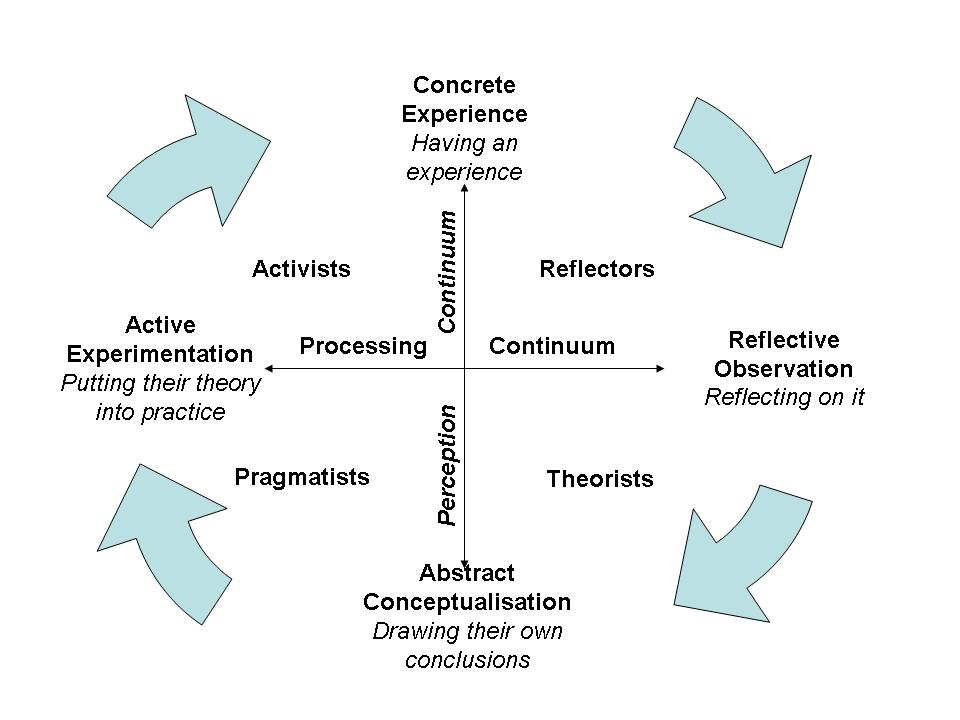
\includegraphics[width=5in]{honey_mumford.jpg}
    \caption{The Honey and Mumford model}
\end{figure}


\paragraph In this model, learners are classified into four groups: reflectors, theorists, pragmatist, activists. Among Computer Science students, it is very easy to find one with particular learning style using Honey and Mumford's model \cite{HoneyMumford}: 
 
\begin{itemize} 
\item Reflectors: They tend to learn by observation or actions. They could learn and view things from many perspectives and come up with many new ideas. As members in a programming project group, they would be recognized as activists in brainstorms, or maybe even a designer in UML (a way to visualize the design of a system in software engineering).
\item Theorists: They tends to learn by abstract concepts, both from textbooks and lectures. They are more likely to behave well when they could follow Functional Design Documents in Computer Science project, as well as to be a good coder. 
\item Pragmatists: They love to get on-hand practice after learning because feedbacks from practice will be valuable to them. They are more likely to choose job careers as Quality Assurance in Computer Science field because being a QA requires to apply rules to actual projects. 
\item Activists: Unlike pragmatists, activists like to try things directly. Thus, they could solve unknown problems in a faster manner. Usually, they will grasp new skills actively, which is a good qualification for a developer.
\end{itemize}






\pagebreak
 
\chapter*{Analysis of My Learning Styles}
\addcontentsline{toc}{chapter}{Analysis of My Learning Style}
\setcounter{chapter}{3}
\setcounter{section}{0}

\paragraph As a computer science, it is very helpful to gain a good understanding of my own learning styles, since the incorporation of preferred learning styles could speed up my learning process. I will use  Honey and Mumford's Learning styles questionnaire(2000) as my exploration approach. 
 
\paragraph Based on Honey and Mumford's Learning styles questionnaire(2000), my preferred learning styles could be retrieved from two continuums: "Processing Continuum: Our approach to a task — learn by doing or watching" and "Perception Continuum: Our emotional response — learn by thinking or feeling". For "Processing Continuum" questions, there are two answers, "doing" or "watching"; For "Perception Continuum" questions, I could choose either "thinking" or "feeling". At the end, I need to add up the number of my statements, and pick the one that has the larger number of choices. 
 
\paragraph I tried the questionnaire two times: First time when I was in an academic term - Spring 2015; Second time when I'm in a co-op term - Fall 2016. I have recorded the results of these two attempts. To my surprise, the results are different. I fell into "watching and thinking - a theorist" for the first time. However, after I began my co-op term, I changed to a "pragmatist - doing and thinking". This proves the statement "preferences for learning styles change over time" (Dunn and Griggs 1995).  
\section {My learning style in school}

\paragraph When I was in school, I really enjoy attending lectures and reading textbooks, because the content from a lecture or a textbook is well organized, I could think and review from time to time which leads to a good understanding. 

\paragraph One impressive lecture experience for me is a lecture about "copy constructor" in CS246. It is a part of Object-oriented programming. In order to explain it clearly, my instructor firstly tell me the background of Object-oriented programming, telling us if we want to clone an object, I need to use  "copy constructor" in our code. Then I got to know there are two kinds of copy constructors, one is called "shallow copy" and one "deep copy", and I need to adopt different copy method in different situations. 

\paragraph The assignment after the lecture is to write short C++ codes of "shallow copy" and "deep copy", which is quite easy after the lecture.   
During the lecture, I kept asking myself: What is Object-oriented programming? Why do I need a "shallow copy" or a "deep copy"? How could I implement it? This experience is really enjoyable, since I don’t have to search anything. I could learn well by following an instructor's ideas, keep thinking, get answer from lecture, and practice. At that time, I was a typical theorist. 

\section {My learning style at work}

\paragraph After I started my co-op work, I realized I changed my way to learn. My supervisors and co-workers would show me how to finish a task by steps in training time, seldom explain to me why I need to go forward by those steps. However, I gained a lot after trying to find the relations of each step, b gathering information from the sequence of steps and observation. Now my critical thinking skills have been improved after half of this co-op term. Now, I will claim to be a pragmatist. 
 
\paragraph Although I changed from a theorist to a pragmatist, critical thinking still domains my learning. I truly value critical thinking in this information-overloaded age, and I will do more to  "develop and effectively apply critical thinking skills to my academic studies, to the complex problems that I will face, and to the critical choices I will be forced to make as a result of the information explosion and other rapid technological changes" (Oliver & Utermohlen, p. 1 1995).

\chapter*{Conclusions and Recommendations}
\addcontentsline{toc}{chapter}{Conclusions and Recommendations}
\setcounter{chapter}{5}
\setcounter{section}{0}

\section{Conclusions} %% at least 3 conclusions

\paragraph A typical learning process of a computer science student could be described by Kolb's four stages learning theories. Some scenes like learning calculus, learning to build a computer and learning to use a new software through a demonstration are analyzed, by separating each scene into four stages.

\paragraph Any stage might be entered firstly to achieve productive learning, as long as all four stages are covered. In the example of learning calculus, “formatting abstract concepts” is accomplished at first, whereas the learning process of building a computer begins with “having a solid experience”.

\paragraph The statement "preferences for learning styles change over time" (Dunn and Griggs 1995) is applicable to the author. By recording the results of answering Honey and Mumford's Learning styles questionnaire at school and at work, a change from "watching and thinking - a theorist" to a "pragmatist - doing and thinking" is found by the author. 

\section{Recommendations} %% at least 2 recommendations


\paragraph This report, titled Learning Styles of a Computer Science Student, provides a short overview of some popular learning styles models and theories in the world, analyzes suitability of Kolb's Model to a computer science student, as well as Honey and Mumford's variation on the Kolb system.

\paragraph Three conclusions are reached in this report. First, a typical learning process of a computer science student could be described by Kolb's four stages learning theories. This is concluded from three common scenes of a computer science student. Second, any stage in a learning model might be entered firstly to achieve productive learning, as long as all four stages are covered. This is gained by extracting the steps of learning process. The author also concluded learning styles will change over time based on the statement from Dunn and Griggs.

\paragraph The author suggests everyone who wants to be a productive learner should check if the learning process covers all four stages. Also it is always a good idea to adopt a most appropriate learning style, since learning conditions and requirements change as the time goes.


\bibliography{references}

\chapter*{Appendices}

Your report must:

\begin{itemize}[label={•	[T] }]
    \item{Include 4-6 pages of body content. Figures or tables that are included in the body are excluded in the 4-6 page count. (Example: 8 pages of content that includes a one-page figure and a half-page table counts as 6.5 pages of body content.) Adherence to the 3Cs (clarity, conciseness, and coherence) will allow you to meet this page limit. }
    \item{Include at least one table (Place the table in the body of your report if you discuss it in detail; place the table in an appendix if your analysis refers to it only briefly.) }
    \item{Include at least one figure (Place the figure in the body of your report if you discuss it in detail; place the figure in an appendix if your analysis refers to it only briefly.) }
    \item{Use a 12-point serif font}
    \item{Be double-spaced}
    \item{Be written in formal, standard English, with no contractions}
    \item{Be spell-checked and proofread}
    \item{Include pages numbered according to the conventions described in the Report Resources tab. }
\end{itemize}

\noindent Your report must conform to the format and conventions described in the Report Resources page. You do not have to bind your report or include a front cover because you will submit your report to us online. Your report will include the following pages and sections:

\begin{itemize}[label={•	[T] }]
    \item{Title page}
    \item{Letter of submittal (addressed to the PD 2 course instructor) }
    \item{Table of content}
    \item{List of figures and tables, if appropriate (Figures or tables in an appendix should not be listed on the List of figures and tables; figures or tables elsewhere in your report are required to be on this list.) }
    \item{Summary }
    \item{Introduction}
    \item{Body (that includes both an objective analytical component and a reflective component) }
    \item{Conclusions (the section is "conclusions" as in "findings", not "conclusion") }
    \item{Recommendations (specific, measurable, and attainable) }
    \item{References }
    \item{Appendices (you need at least one appendix which includes this checklist) }
\end{itemize}

\end{document}
